\documentclass[]{article}
\usepackage{lmodern}
\usepackage{amssymb,amsmath}
\usepackage{ifxetex,ifluatex}
\usepackage{fixltx2e} % provides \textsubscript
\ifnum 0\ifxetex 1\fi\ifluatex 1\fi=0 % if pdftex
  \usepackage[T1]{fontenc}
  \usepackage[utf8]{inputenc}
\else % if luatex or xelatex
  \ifxetex
    \usepackage{mathspec}
  \else
    \usepackage{fontspec}
  \fi
  \defaultfontfeatures{Ligatures=TeX,Scale=MatchLowercase}
\fi
% use upquote if available, for straight quotes in verbatim environments
\IfFileExists{upquote.sty}{\usepackage{upquote}}{}
% use microtype if available
\IfFileExists{microtype.sty}{%
\usepackage{microtype}
\UseMicrotypeSet[protrusion]{basicmath} % disable protrusion for tt fonts
}{}
\usepackage[margin=1in]{geometry}
\usepackage{hyperref}
\hypersetup{unicode=true,
            pdftitle={hw4},
            pdfauthor={Kaicheng Luo},
            pdfborder={0 0 0},
            breaklinks=true}
\urlstyle{same}  % don't use monospace font for urls
\usepackage{color}
\usepackage{fancyvrb}
\newcommand{\VerbBar}{|}
\newcommand{\VERB}{\Verb[commandchars=\\\{\}]}
\DefineVerbatimEnvironment{Highlighting}{Verbatim}{commandchars=\\\{\}}
% Add ',fontsize=\small' for more characters per line
\usepackage{framed}
\definecolor{shadecolor}{RGB}{248,248,248}
\newenvironment{Shaded}{\begin{snugshade}}{\end{snugshade}}
\newcommand{\KeywordTok}[1]{\textcolor[rgb]{0.13,0.29,0.53}{\textbf{#1}}}
\newcommand{\DataTypeTok}[1]{\textcolor[rgb]{0.13,0.29,0.53}{#1}}
\newcommand{\DecValTok}[1]{\textcolor[rgb]{0.00,0.00,0.81}{#1}}
\newcommand{\BaseNTok}[1]{\textcolor[rgb]{0.00,0.00,0.81}{#1}}
\newcommand{\FloatTok}[1]{\textcolor[rgb]{0.00,0.00,0.81}{#1}}
\newcommand{\ConstantTok}[1]{\textcolor[rgb]{0.00,0.00,0.00}{#1}}
\newcommand{\CharTok}[1]{\textcolor[rgb]{0.31,0.60,0.02}{#1}}
\newcommand{\SpecialCharTok}[1]{\textcolor[rgb]{0.00,0.00,0.00}{#1}}
\newcommand{\StringTok}[1]{\textcolor[rgb]{0.31,0.60,0.02}{#1}}
\newcommand{\VerbatimStringTok}[1]{\textcolor[rgb]{0.31,0.60,0.02}{#1}}
\newcommand{\SpecialStringTok}[1]{\textcolor[rgb]{0.31,0.60,0.02}{#1}}
\newcommand{\ImportTok}[1]{#1}
\newcommand{\CommentTok}[1]{\textcolor[rgb]{0.56,0.35,0.01}{\textit{#1}}}
\newcommand{\DocumentationTok}[1]{\textcolor[rgb]{0.56,0.35,0.01}{\textbf{\textit{#1}}}}
\newcommand{\AnnotationTok}[1]{\textcolor[rgb]{0.56,0.35,0.01}{\textbf{\textit{#1}}}}
\newcommand{\CommentVarTok}[1]{\textcolor[rgb]{0.56,0.35,0.01}{\textbf{\textit{#1}}}}
\newcommand{\OtherTok}[1]{\textcolor[rgb]{0.56,0.35,0.01}{#1}}
\newcommand{\FunctionTok}[1]{\textcolor[rgb]{0.00,0.00,0.00}{#1}}
\newcommand{\VariableTok}[1]{\textcolor[rgb]{0.00,0.00,0.00}{#1}}
\newcommand{\ControlFlowTok}[1]{\textcolor[rgb]{0.13,0.29,0.53}{\textbf{#1}}}
\newcommand{\OperatorTok}[1]{\textcolor[rgb]{0.81,0.36,0.00}{\textbf{#1}}}
\newcommand{\BuiltInTok}[1]{#1}
\newcommand{\ExtensionTok}[1]{#1}
\newcommand{\PreprocessorTok}[1]{\textcolor[rgb]{0.56,0.35,0.01}{\textit{#1}}}
\newcommand{\AttributeTok}[1]{\textcolor[rgb]{0.77,0.63,0.00}{#1}}
\newcommand{\RegionMarkerTok}[1]{#1}
\newcommand{\InformationTok}[1]{\textcolor[rgb]{0.56,0.35,0.01}{\textbf{\textit{#1}}}}
\newcommand{\WarningTok}[1]{\textcolor[rgb]{0.56,0.35,0.01}{\textbf{\textit{#1}}}}
\newcommand{\AlertTok}[1]{\textcolor[rgb]{0.94,0.16,0.16}{#1}}
\newcommand{\ErrorTok}[1]{\textcolor[rgb]{0.64,0.00,0.00}{\textbf{#1}}}
\newcommand{\NormalTok}[1]{#1}
\usepackage{graphicx,grffile}
\makeatletter
\def\maxwidth{\ifdim\Gin@nat@width>\linewidth\linewidth\else\Gin@nat@width\fi}
\def\maxheight{\ifdim\Gin@nat@height>\textheight\textheight\else\Gin@nat@height\fi}
\makeatother
% Scale images if necessary, so that they will not overflow the page
% margins by default, and it is still possible to overwrite the defaults
% using explicit options in \includegraphics[width, height, ...]{}
\setkeys{Gin}{width=\maxwidth,height=\maxheight,keepaspectratio}
\IfFileExists{parskip.sty}{%
\usepackage{parskip}
}{% else
\setlength{\parindent}{0pt}
\setlength{\parskip}{6pt plus 2pt minus 1pt}
}
\setlength{\emergencystretch}{3em}  % prevent overfull lines
\providecommand{\tightlist}{%
  \setlength{\itemsep}{0pt}\setlength{\parskip}{0pt}}
\setcounter{secnumdepth}{0}
% Redefines (sub)paragraphs to behave more like sections
\ifx\paragraph\undefined\else
\let\oldparagraph\paragraph
\renewcommand{\paragraph}[1]{\oldparagraph{#1}\mbox{}}
\fi
\ifx\subparagraph\undefined\else
\let\oldsubparagraph\subparagraph
\renewcommand{\subparagraph}[1]{\oldsubparagraph{#1}\mbox{}}
\fi

%%% Use protect on footnotes to avoid problems with footnotes in titles
\let\rmarkdownfootnote\footnote%
\def\footnote{\protect\rmarkdownfootnote}

%%% Change title format to be more compact
\usepackage{titling}

% Create subtitle command for use in maketitle
\providecommand{\subtitle}[1]{
  \posttitle{
    \begin{center}\large#1\end{center}
    }
}

\setlength{\droptitle}{-2em}

  \title{hw4}
    \pretitle{\vspace{\droptitle}\centering\huge}
  \posttitle{\par}
    \author{Kaicheng Luo}
    \preauthor{\centering\large\emph}
  \postauthor{\par}
      \predate{\centering\large\emph}
  \postdate{\par}
    \date{2019/9/30}


\begin{document}
\maketitle

Simulation

\begin{Shaded}
\begin{Highlighting}[]
\CommentTok{# Model H0: y = coef_0}
\CommentTok{# Model H1: y = coef_1a + coef_1b}
\NormalTok{n_out <-}\StringTok{ }\DecValTok{20000}
\NormalTok{epsilon <-}\StringTok{ }\DecValTok{0}

\CommentTok{# For each iteration, I'd like to record the following values}
\NormalTok{coef_}\DecValTok{0}\NormalTok{ <-}\StringTok{ }\KeywordTok{vector}\NormalTok{()}
\NormalTok{coef_1a <-}\StringTok{ }\KeywordTok{vector}\NormalTok{()}
\NormalTok{coef_1b <-}\StringTok{ }\KeywordTok{vector}\NormalTok{()}
\NormalTok{MSE_}\DecValTok{0}\NormalTok{ <-}\StringTok{ }\KeywordTok{rep}\NormalTok{(}\DecValTok{0}\NormalTok{, }\DecValTok{500}\NormalTok{)}
\NormalTok{MSE_}\DecValTok{1}\NormalTok{ <-}\StringTok{ }\KeywordTok{rep}\NormalTok{(}\DecValTok{0}\NormalTok{, }\DecValTok{500}\NormalTok{)}

\CommentTok{# Here we randomly draw a test set}
\KeywordTok{set.seed}\NormalTok{(}\DecValTok{12345}\NormalTok{)}
\NormalTok{x_out <-}\StringTok{ }\KeywordTok{runif}\NormalTok{(n_out, }\DataTypeTok{min =} \OperatorTok{-}\DecValTok{1}\NormalTok{, }\DataTypeTok{max =} \DecValTok{1}\NormalTok{)}
\NormalTok{y_out <-}\StringTok{ }\NormalTok{x_out}\OperatorTok{^}\DecValTok{2} \OperatorTok{+}\StringTok{ }\NormalTok{epsilon}

\CommentTok{# Fit the model with 2 training sets, and calculate the MSE of each model we fit}
\ControlFlowTok{for}\NormalTok{ (i }\ControlFlowTok{in} \DecValTok{1}\OperatorTok{:}\DecValTok{500}\NormalTok{)\{}
\NormalTok{  x <-}\StringTok{ }\KeywordTok{runif}\NormalTok{(}\DataTypeTok{n =} \DecValTok{2}\NormalTok{, }\DataTypeTok{min =} \OperatorTok{-}\DecValTok{1}\NormalTok{, }\DataTypeTok{max =} \DecValTok{1}\NormalTok{)}
\NormalTok{  y <-}\StringTok{ }\NormalTok{x}\OperatorTok{^}\DecValTok{2} \OperatorTok{+}\StringTok{ }\NormalTok{epsilon}
\NormalTok{  coef_}\DecValTok{0}\NormalTok{ <-}\StringTok{ }\KeywordTok{c}\NormalTok{(coef_}\DecValTok{0}\NormalTok{, (y[}\DecValTok{1}\NormalTok{]}\OperatorTok{+}\NormalTok{y[}\DecValTok{2}\NormalTok{])}\OperatorTok{/}\DecValTok{2}\NormalTok{)}
\NormalTok{  coef_1a <-}\StringTok{ }\KeywordTok{c}\NormalTok{(coef_1a, y[}\DecValTok{1}\NormalTok{] }\OperatorTok{-}\StringTok{ }\NormalTok{x[}\DecValTok{1}\NormalTok{]}\OperatorTok{*}\NormalTok{(y[}\DecValTok{2}\NormalTok{]}\OperatorTok{-}\NormalTok{y[}\DecValTok{1}\NormalTok{])}\OperatorTok{/}\NormalTok{(x[}\DecValTok{2}\NormalTok{]}\OperatorTok{-}\NormalTok{x[}\DecValTok{1}\NormalTok{]))}
\NormalTok{  coef_1b <-}\StringTok{ }\KeywordTok{c}\NormalTok{(coef_1b, (y[}\DecValTok{2}\NormalTok{]}\OperatorTok{-}\NormalTok{y[}\DecValTok{1}\NormalTok{])}\OperatorTok{/}\NormalTok{(x[}\DecValTok{2}\NormalTok{]}\OperatorTok{-}\NormalTok{x[}\DecValTok{1}\NormalTok{]))}
  \ControlFlowTok{for}\NormalTok{ (j }\ControlFlowTok{in} \DecValTok{1}\OperatorTok{:}\NormalTok{n_out)\{}
\NormalTok{    MSE_}\DecValTok{0}\NormalTok{[i] =}\StringTok{ }\NormalTok{MSE_}\DecValTok{0}\NormalTok{[i] }\OperatorTok{+}\StringTok{ }\NormalTok{((y_out[j] }\OperatorTok{-}\StringTok{ }\NormalTok{coef_}\DecValTok{0}\NormalTok{[i])}\OperatorTok{^}\DecValTok{2}\NormalTok{)}\OperatorTok{/}\NormalTok{n_out}
\NormalTok{    MSE_}\DecValTok{1}\NormalTok{[i] =}\StringTok{ }\NormalTok{MSE_}\DecValTok{1}\NormalTok{[i] }\OperatorTok{+}\StringTok{ }\NormalTok{((y_out[j] }\OperatorTok{-}\StringTok{ }\NormalTok{coef_1a[i] }\OperatorTok{-}\StringTok{ }\NormalTok{coef_1b[i] }\OperatorTok{*}\StringTok{ }\NormalTok{x_out[j])}\OperatorTok{^}\DecValTok{2}\NormalTok{)}\OperatorTok{/}\NormalTok{n_out}
\NormalTok{  \}}
\NormalTok{\}}
\end{Highlighting}
\end{Shaded}

\begin{Shaded}
\begin{Highlighting}[]
\CommentTok{# Here's the code for the H_0 plot}
\NormalTok{plot_data <-}\StringTok{ }\KeywordTok{data.frame}\NormalTok{(}\DataTypeTok{x =}\NormalTok{ x_out, }\DataTypeTok{y =}\NormalTok{ y_out)}
\NormalTok{plot_data }\OperatorTok
\StringTok{  }\KeywordTok{ggplot}\NormalTok{() }\OperatorTok{+}\StringTok{ }\KeywordTok{theme_bw}\NormalTok{() }\OperatorTok{+}
\StringTok{  }\KeywordTok{geom_smooth}\NormalTok{(}\KeywordTok{aes}\NormalTok{(}\DataTypeTok{x =}\NormalTok{ x, }\DataTypeTok{y =}\NormalTok{ y), }\DataTypeTok{color =} \StringTok{'blue'}\NormalTok{) }\OperatorTok{+}
\StringTok{  }\KeywordTok{geom_hline}\NormalTok{(}\DataTypeTok{yintercept =}\NormalTok{ coef_}\DecValTok{0}\NormalTok{, }\DataTypeTok{alpha =} \FloatTok{0.05}\NormalTok{) }\OperatorTok{+}
\StringTok{  }\KeywordTok{geom_hline}\NormalTok{(}\DataTypeTok{yintercept =} \KeywordTok{mean}\NormalTok{(coef_}\DecValTok{0}\NormalTok{), }\DataTypeTok{color =} \StringTok{'red'}\NormalTok{, }\DataTypeTok{size =} \DecValTok{1}\NormalTok{) }\OperatorTok{+}
\StringTok{  }\KeywordTok{scale_y_continuous}\NormalTok{(}\DataTypeTok{expand =} \KeywordTok{c}\NormalTok{(}\FloatTok{0.001}\NormalTok{, }\FloatTok{0.001}\NormalTok{)) }\OperatorTok{+}
\StringTok{  }\KeywordTok{scale_x_continuous}\NormalTok{(}\DataTypeTok{expand =} \KeywordTok{c}\NormalTok{(}\FloatTok{0.001}\NormalTok{, }\FloatTok{0.001}\NormalTok{)) }\OperatorTok{+}
\StringTok{  }\KeywordTok{labs}\NormalTok{(}
    \DataTypeTok{title =} \StringTok{"Hypothesis 0"}
\NormalTok{  )}
\end{Highlighting}
\end{Shaded}

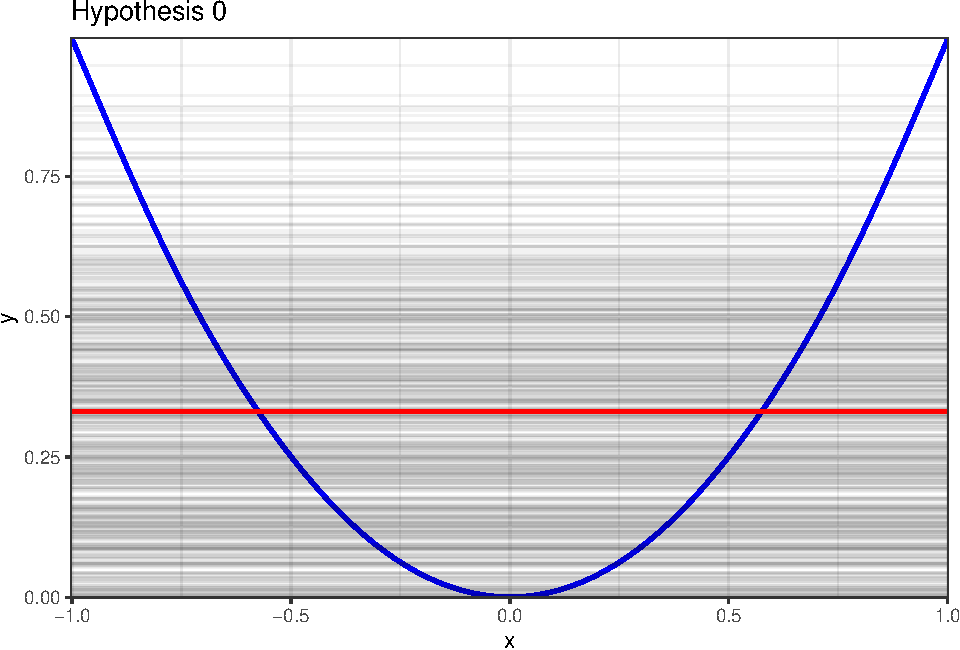
\includegraphics{hw4_files/figure-latex/unnamed-chunk-2-1.pdf}

\begin{Shaded}
\begin{Highlighting}[]
\CommentTok{# Here's the code for the H_1 plot}
\NormalTok{plot_data }\OperatorTok
\StringTok{  }\KeywordTok{ggplot}\NormalTok{() }\OperatorTok{+}\StringTok{ }\KeywordTok{theme_bw}\NormalTok{() }\OperatorTok{+}
\StringTok{  }\KeywordTok{geom_smooth}\NormalTok{(}\KeywordTok{aes}\NormalTok{(}\DataTypeTok{x =}\NormalTok{ x, }\DataTypeTok{y =}\NormalTok{ y), }\DataTypeTok{color =} \StringTok{'blue'}\NormalTok{) }\OperatorTok{+}
\StringTok{  }\KeywordTok{geom_abline}\NormalTok{(}\DataTypeTok{intercept =}\NormalTok{ coef_1a, }\DataTypeTok{slope =}\NormalTok{ coef_1b, }\DataTypeTok{alpha =} \FloatTok{0.1}\NormalTok{) }\OperatorTok{+}
\StringTok{  }\KeywordTok{geom_abline}\NormalTok{(}\DataTypeTok{intercept =} \KeywordTok{mean}\NormalTok{(coef_1a), }\DataTypeTok{slope =} \KeywordTok{mean}\NormalTok{(coef_1b), }\DataTypeTok{color =} \StringTok{'red'}\NormalTok{, }\DataTypeTok{size =} \DecValTok{1}\NormalTok{) }\OperatorTok{+}
\StringTok{  }\KeywordTok{scale_y_continuous}\NormalTok{(}\DataTypeTok{expand =} \KeywordTok{c}\NormalTok{(}\FloatTok{0.001}\NormalTok{, }\FloatTok{0.001}\NormalTok{)) }\OperatorTok{+}
\StringTok{  }\KeywordTok{scale_x_continuous}\NormalTok{(}\DataTypeTok{expand =} \KeywordTok{c}\NormalTok{(}\FloatTok{0.001}\NormalTok{, }\FloatTok{0.001}\NormalTok{)) }\OperatorTok{+}
\StringTok{  }\KeywordTok{labs}\NormalTok{(}
    \DataTypeTok{title =} \StringTok{"Hypothesis 1"}
\NormalTok{  )}
\end{Highlighting}
\end{Shaded}

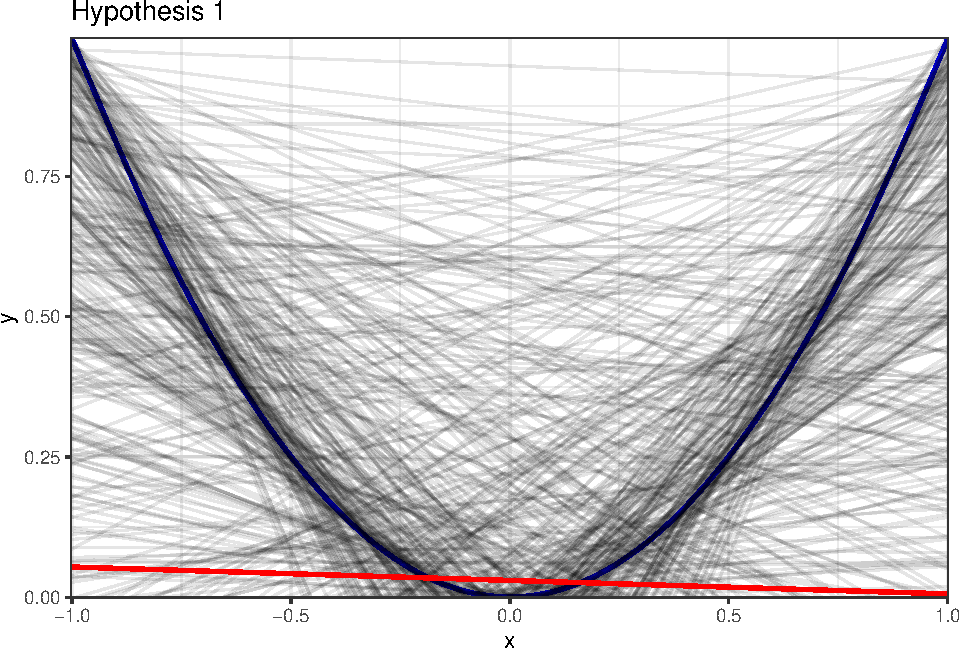
\includegraphics{hw4_files/figure-latex/unnamed-chunk-3-1.pdf}

\begin{Shaded}
\begin{Highlighting}[]
\CommentTok{# To verify the bias-variance trade-off rigorously, we examine the first model}
\NormalTok{OverallMSE_}\DecValTok{0}\NormalTok{ <-}\StringTok{ }\KeywordTok{mean}\NormalTok{(MSE_}\DecValTok{0}\NormalTok{)}
\NormalTok{bias <-}\StringTok{ }\KeywordTok{vector}\NormalTok{()}
\NormalTok{variance <-}\StringTok{ }\KeywordTok{vector}\NormalTok{()}
\ControlFlowTok{for}\NormalTok{ (i }\ControlFlowTok{in} \DecValTok{1}\OperatorTok{:}\DecValTok{20000}\NormalTok{)\{}
\NormalTok{  bias[i] <-}\StringTok{ }\NormalTok{(}\KeywordTok{mean}\NormalTok{(coef_}\DecValTok{0}\NormalTok{) }\OperatorTok{-}\StringTok{ }\NormalTok{y_out[i])}\OperatorTok{^}\DecValTok{2}
\NormalTok{\}}
\NormalTok{bias_}\DecValTok{0}\NormalTok{ <-}\StringTok{ }\KeywordTok{mean}\NormalTok{(bias)}
\ControlFlowTok{for}\NormalTok{ (i }\ControlFlowTok{in} \DecValTok{1}\OperatorTok{:}\DecValTok{500}\NormalTok{)\{}
\NormalTok{  variance[i] <-}\StringTok{ }\NormalTok{(}\KeywordTok{mean}\NormalTok{(coef_}\DecValTok{0}\NormalTok{) }\OperatorTok{-}\StringTok{ }\NormalTok{coef_}\DecValTok{0}\NormalTok{[i])}\OperatorTok{^}\DecValTok{2}
\NormalTok{\}}
\NormalTok{variance_}\DecValTok{0}\NormalTok{ <-}\StringTok{ }\KeywordTok{mean}\NormalTok{(variance)}
\CommentTok{# Display it tidily}
\NormalTok{model_}\DecValTok{0}\NormalTok{ <-}\StringTok{ }\KeywordTok{data.frame}\NormalTok{(}\StringTok{"OverallMSE"}\NormalTok{ =}\StringTok{ }\NormalTok{OverallMSE_}\DecValTok{0}\NormalTok{, }\StringTok{"Bias"}\NormalTok{ =}\StringTok{ }\NormalTok{bias_}\DecValTok{0}\NormalTok{, }\StringTok{"Var"}\NormalTok{ =}\StringTok{ }\NormalTok{variance_}\DecValTok{0}\NormalTok{)}
\NormalTok{model_}\DecValTok{0}
\end{Highlighting}
\end{Shaded}

\begin{verbatim}
##   OverallMSE       Bias        Var
## 1  0.1330587 0.08903894 0.04401978
\end{verbatim}

\begin{Shaded}
\begin{Highlighting}[]
\CommentTok{# If the decomposition is correct, it shall return 0}
\NormalTok{model_}\DecValTok{0}\OperatorTok{$}\NormalTok{OverallMSE }\OperatorTok{-}\StringTok{ }\NormalTok{model_}\DecValTok{0}\OperatorTok{$}\NormalTok{Bias }\OperatorTok{-}\StringTok{ }\NormalTok{model_}\DecValTok{0}\OperatorTok{$}\NormalTok{Var}
\end{Highlighting}
\end{Shaded}

\begin{verbatim}
## [1] 6.938894e-18
\end{verbatim}

\begin{Shaded}
\begin{Highlighting}[]
\CommentTok{# Similarly, we can do this to the second model}
\NormalTok{OverallMSE_}\DecValTok{1}\NormalTok{ <-}\StringTok{ }\KeywordTok{mean}\NormalTok{(MSE_}\DecValTok{1}\NormalTok{)}
\NormalTok{bias <-}\StringTok{ }\KeywordTok{vector}\NormalTok{()}
\NormalTok{variance <-}\StringTok{ }\KeywordTok{rep}\NormalTok{(}\DecValTok{0}\NormalTok{, n_out)}
\ControlFlowTok{for}\NormalTok{ (i }\ControlFlowTok{in} \DecValTok{1}\OperatorTok{:}\DecValTok{20000}\NormalTok{)\{}
\NormalTok{  bias[i] <-}\StringTok{ }\NormalTok{(}\KeywordTok{mean}\NormalTok{(coef_1a) }\OperatorTok{+}\StringTok{ }\KeywordTok{mean}\NormalTok{(coef_1b)}\OperatorTok{*}\NormalTok{x_out[i] }\OperatorTok{-}\StringTok{ }\NormalTok{y_out[i])}\OperatorTok{^}\DecValTok{2}
\NormalTok{\}}
\NormalTok{bias_}\DecValTok{1}\NormalTok{ <-}\StringTok{ }\KeywordTok{mean}\NormalTok{(bias)}
\ControlFlowTok{for}\NormalTok{ (i }\ControlFlowTok{in} \DecValTok{1}\OperatorTok{:}\DecValTok{500}\NormalTok{)\{}
  \ControlFlowTok{for}\NormalTok{ (j }\ControlFlowTok{in} \DecValTok{1}\OperatorTok{:}\NormalTok{n_out)\{}
\NormalTok{    variance[i] =}\StringTok{ }\NormalTok{variance[i] }\OperatorTok{+}\StringTok{ }\NormalTok{((}\KeywordTok{mean}\NormalTok{(coef_1a) }\OperatorTok{+}\StringTok{ }\KeywordTok{mean}\NormalTok{(coef_1b)}\OperatorTok{*}\NormalTok{x_out[j] }\OperatorTok{-}\StringTok{ }\NormalTok{coef_1a[i] }\OperatorTok{-}\StringTok{ }\NormalTok{coef_1b[i]}\OperatorTok{*}\NormalTok{x_out[j])}\OperatorTok{^}\DecValTok{2}\NormalTok{)}\OperatorTok{/}\DecValTok{500}
\NormalTok{  \}}
\NormalTok{\}}

\NormalTok{variance_}\DecValTok{1}\NormalTok{ <-}\StringTok{ }\KeywordTok{mean}\NormalTok{(variance)}
\CommentTok{# Display it tidily}
\NormalTok{model_}\DecValTok{1}\NormalTok{ <-}\StringTok{ }\KeywordTok{data.frame}\NormalTok{(}\StringTok{"OverallMSE"}\NormalTok{ =}\StringTok{ }\NormalTok{OverallMSE_}\DecValTok{1}\NormalTok{, }\StringTok{"Bias"}\NormalTok{ =}\StringTok{ }\NormalTok{bias_}\DecValTok{1}\NormalTok{, }\StringTok{"Var"}\NormalTok{ =}\StringTok{ }\NormalTok{variance_}\DecValTok{1}\NormalTok{)}
\NormalTok{model_}\DecValTok{1}
\end{Highlighting}
\end{Shaded}

\begin{verbatim}
##   OverallMSE      Bias       Var
## 1   0.486243 0.1802108 0.3060323
\end{verbatim}

\begin{Shaded}
\begin{Highlighting}[]
\CommentTok{# If the decomposition is correct, it shall return 0}
\NormalTok{model_}\DecValTok{1}\OperatorTok{$}\NormalTok{OverallMSE }\OperatorTok{-}\StringTok{ }\NormalTok{model_}\DecValTok{1}\OperatorTok{$}\NormalTok{Bias }\OperatorTok{-}\StringTok{ }\NormalTok{model_}\DecValTok{1}\OperatorTok{$}\NormalTok{Var}
\end{Highlighting}
\end{Shaded}

\begin{verbatim}
## [1] 0
\end{verbatim}

Run another simulation with noise

\begin{Shaded}
\begin{Highlighting}[]
\CommentTok{# Model H0: y = coef_0}
\CommentTok{# Model H1: y = coef_1a + coef_1b}
\NormalTok{n_out <-}\StringTok{ }\DecValTok{20000}
\NormalTok{epsilon <-}\StringTok{ }\KeywordTok{rnorm}\NormalTok{(n_out, }\DecValTok{0}\NormalTok{, }\FloatTok{0.1}\NormalTok{)}

\CommentTok{# For each iteration, I'd like to record the following values}
\NormalTok{coef_}\DecValTok{0}\NormalTok{ <-}\StringTok{ }\KeywordTok{vector}\NormalTok{()}
\NormalTok{coef_1a <-}\StringTok{ }\KeywordTok{vector}\NormalTok{()}
\NormalTok{coef_1b <-}\StringTok{ }\KeywordTok{vector}\NormalTok{()}
\NormalTok{MSE_}\DecValTok{0}\NormalTok{ <-}\StringTok{ }\KeywordTok{rep}\NormalTok{(}\DecValTok{0}\NormalTok{, }\DecValTok{500}\NormalTok{)}
\NormalTok{MSE_}\DecValTok{1}\NormalTok{ <-}\StringTok{ }\KeywordTok{rep}\NormalTok{(}\DecValTok{0}\NormalTok{, }\DecValTok{500}\NormalTok{)}

\CommentTok{# Here we randomly draw a test set}
\KeywordTok{set.seed}\NormalTok{(}\DecValTok{12345}\NormalTok{)}
\NormalTok{x_out <-}\StringTok{ }\KeywordTok{runif}\NormalTok{(n_out, }\DataTypeTok{min =} \OperatorTok{-}\DecValTok{1}\NormalTok{, }\DataTypeTok{max =} \DecValTok{1}\NormalTok{)}
\NormalTok{y_out <-}\StringTok{ }\NormalTok{x_out}\OperatorTok{^}\DecValTok{2} \OperatorTok{+}\StringTok{ }\NormalTok{epsilon}

\CommentTok{# Fit the model with 2 training sets, and calculate the MSE of each model we fit}
\ControlFlowTok{for}\NormalTok{ (i }\ControlFlowTok{in} \DecValTok{1}\OperatorTok{:}\DecValTok{500}\NormalTok{)\{}
\NormalTok{  x <-}\StringTok{ }\KeywordTok{runif}\NormalTok{(}\DataTypeTok{n =} \DecValTok{2}\NormalTok{, }\DataTypeTok{min =} \OperatorTok{-}\DecValTok{1}\NormalTok{, }\DataTypeTok{max =} \DecValTok{1}\NormalTok{)}
\NormalTok{  y <-}\StringTok{ }\NormalTok{x}\OperatorTok{^}\DecValTok{2} \OperatorTok{+}\StringTok{ }\NormalTok{epsilon}
\NormalTok{  coef_}\DecValTok{0}\NormalTok{ <-}\StringTok{ }\KeywordTok{c}\NormalTok{(coef_}\DecValTok{0}\NormalTok{, (y[}\DecValTok{1}\NormalTok{]}\OperatorTok{+}\NormalTok{y[}\DecValTok{2}\NormalTok{])}\OperatorTok{/}\DecValTok{2}\NormalTok{)}
\NormalTok{  coef_1a <-}\StringTok{ }\KeywordTok{c}\NormalTok{(coef_1a, y[}\DecValTok{1}\NormalTok{] }\OperatorTok{-}\StringTok{ }\NormalTok{x[}\DecValTok{1}\NormalTok{]}\OperatorTok{*}\NormalTok{(y[}\DecValTok{2}\NormalTok{]}\OperatorTok{-}\NormalTok{y[}\DecValTok{1}\NormalTok{])}\OperatorTok{/}\NormalTok{(x[}\DecValTok{2}\NormalTok{]}\OperatorTok{-}\NormalTok{x[}\DecValTok{1}\NormalTok{]))}
\NormalTok{  coef_1b <-}\StringTok{ }\KeywordTok{c}\NormalTok{(coef_1b, (y[}\DecValTok{2}\NormalTok{]}\OperatorTok{-}\NormalTok{y[}\DecValTok{1}\NormalTok{])}\OperatorTok{/}\NormalTok{(x[}\DecValTok{2}\NormalTok{]}\OperatorTok{-}\NormalTok{x[}\DecValTok{1}\NormalTok{]))}
  \ControlFlowTok{for}\NormalTok{ (j }\ControlFlowTok{in} \DecValTok{1}\OperatorTok{:}\NormalTok{n_out)\{}
\NormalTok{    MSE_}\DecValTok{0}\NormalTok{[i] =}\StringTok{ }\NormalTok{MSE_}\DecValTok{0}\NormalTok{[i] }\OperatorTok{+}\StringTok{ }\NormalTok{((y_out[j] }\OperatorTok{-}\StringTok{ }\NormalTok{coef_}\DecValTok{0}\NormalTok{[i])}\OperatorTok{^}\DecValTok{2}\NormalTok{)}\OperatorTok{/}\NormalTok{n_out}
\NormalTok{    MSE_}\DecValTok{1}\NormalTok{[i] =}\StringTok{ }\NormalTok{MSE_}\DecValTok{1}\NormalTok{[i] }\OperatorTok{+}\StringTok{ }\NormalTok{((y_out[j] }\OperatorTok{-}\StringTok{ }\NormalTok{coef_1a[i] }\OperatorTok{-}\StringTok{ }\NormalTok{coef_1b[i] }\OperatorTok{*}\StringTok{ }\NormalTok{x_out[j])}\OperatorTok{^}\DecValTok{2}\NormalTok{)}\OperatorTok{/}\NormalTok{n_out}
\NormalTok{  \}}
\NormalTok{\}}
\end{Highlighting}
\end{Shaded}

\begin{Shaded}
\begin{Highlighting}[]
\CommentTok{# Here's the code for the H_0 plot}
\NormalTok{plot_data <-}\StringTok{ }\KeywordTok{data.frame}\NormalTok{(}\DataTypeTok{x =}\NormalTok{ x_out, }\DataTypeTok{y =}\NormalTok{ y_out)}
\NormalTok{plot_data }\OperatorTok
\StringTok{  }\KeywordTok{ggplot}\NormalTok{() }\OperatorTok{+}\StringTok{ }\KeywordTok{theme_bw}\NormalTok{() }\OperatorTok{+}
\StringTok{  }\KeywordTok{geom_point}\NormalTok{(}\KeywordTok{aes}\NormalTok{(}\DataTypeTok{x =}\NormalTok{ x, }\DataTypeTok{y =}\NormalTok{ y), }\DataTypeTok{color =} \StringTok{'blue'}\NormalTok{, }\DataTypeTok{alpha =} \FloatTok{0.02}\NormalTok{) }\OperatorTok{+}
\StringTok{  }\KeywordTok{geom_smooth}\NormalTok{(}\KeywordTok{aes}\NormalTok{(}\DataTypeTok{x =}\NormalTok{ x, }\DataTypeTok{y =}\NormalTok{ y), }\DataTypeTok{color =} \StringTok{'blue'}\NormalTok{) }\OperatorTok{+}
\StringTok{  }\KeywordTok{geom_hline}\NormalTok{(}\DataTypeTok{yintercept =}\NormalTok{ coef_}\DecValTok{0}\NormalTok{, }\DataTypeTok{alpha =} \FloatTok{0.05}\NormalTok{) }\OperatorTok{+}
\StringTok{  }\KeywordTok{geom_hline}\NormalTok{(}\DataTypeTok{yintercept =} \KeywordTok{mean}\NormalTok{(coef_}\DecValTok{0}\NormalTok{), }\DataTypeTok{color =} \StringTok{'red'}\NormalTok{, }\DataTypeTok{size =} \DecValTok{1}\NormalTok{) }\OperatorTok{+}
\StringTok{  }\KeywordTok{scale_y_continuous}\NormalTok{(}\DataTypeTok{expand =} \KeywordTok{c}\NormalTok{(}\FloatTok{0.001}\NormalTok{, }\FloatTok{0.001}\NormalTok{)) }\OperatorTok{+}
\StringTok{  }\KeywordTok{scale_x_continuous}\NormalTok{(}\DataTypeTok{expand =} \KeywordTok{c}\NormalTok{(}\FloatTok{0.001}\NormalTok{, }\FloatTok{0.001}\NormalTok{)) }\OperatorTok{+}
\StringTok{  }\KeywordTok{labs}\NormalTok{(}
    \DataTypeTok{title =} \StringTok{"Hypothesis 0"}
\NormalTok{  )}
\end{Highlighting}
\end{Shaded}

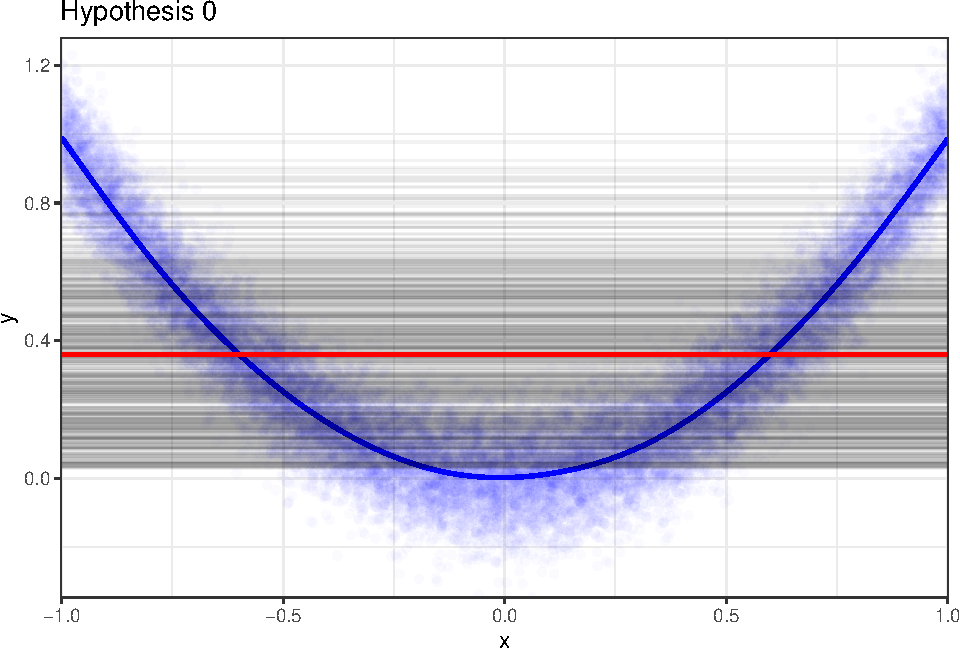
\includegraphics{hw4_files/figure-latex/unnamed-chunk-7-1.pdf}

\begin{Shaded}
\begin{Highlighting}[]
\CommentTok{# Here's the code for the H_1 plot}
\NormalTok{plot_data }\OperatorTok
\StringTok{  }\KeywordTok{ggplot}\NormalTok{() }\OperatorTok{+}\StringTok{ }\KeywordTok{theme_bw}\NormalTok{() }\OperatorTok{+}
\StringTok{  }\KeywordTok{geom_smooth}\NormalTok{(}\KeywordTok{aes}\NormalTok{(}\DataTypeTok{x =}\NormalTok{ x, }\DataTypeTok{y =}\NormalTok{ y), }\DataTypeTok{color =} \StringTok{'blue'}\NormalTok{) }\OperatorTok{+}
\StringTok{  }\KeywordTok{geom_point}\NormalTok{(}\KeywordTok{aes}\NormalTok{(}\DataTypeTok{x =}\NormalTok{ x, }\DataTypeTok{y =}\NormalTok{ y), }\DataTypeTok{color =} \StringTok{'blue'}\NormalTok{, }\DataTypeTok{alpha =} \FloatTok{0.02}\NormalTok{) }\OperatorTok{+}
\StringTok{  }\KeywordTok{geom_abline}\NormalTok{(}\DataTypeTok{intercept =}\NormalTok{ coef_1a, }\DataTypeTok{slope =}\NormalTok{ coef_1b, }\DataTypeTok{alpha =} \FloatTok{0.05}\NormalTok{) }\OperatorTok{+}
\StringTok{  }\KeywordTok{geom_abline}\NormalTok{(}\DataTypeTok{intercept =} \KeywordTok{mean}\NormalTok{(coef_1a), }\DataTypeTok{slope =} \KeywordTok{mean}\NormalTok{(coef_1b), }\DataTypeTok{color =} \StringTok{'red'}\NormalTok{, }\DataTypeTok{size =} \DecValTok{1}\NormalTok{) }\OperatorTok{+}
\StringTok{  }\KeywordTok{scale_y_continuous}\NormalTok{(}\DataTypeTok{expand =} \KeywordTok{c}\NormalTok{(}\FloatTok{0.001}\NormalTok{, }\FloatTok{0.001}\NormalTok{)) }\OperatorTok{+}
\StringTok{  }\KeywordTok{scale_x_continuous}\NormalTok{(}\DataTypeTok{expand =} \KeywordTok{c}\NormalTok{(}\FloatTok{0.001}\NormalTok{, }\FloatTok{0.001}\NormalTok{)) }\OperatorTok{+}
\StringTok{  }\KeywordTok{labs}\NormalTok{(}
    \DataTypeTok{title =} \StringTok{"Hypothesis 1"}
\NormalTok{  )}
\end{Highlighting}
\end{Shaded}

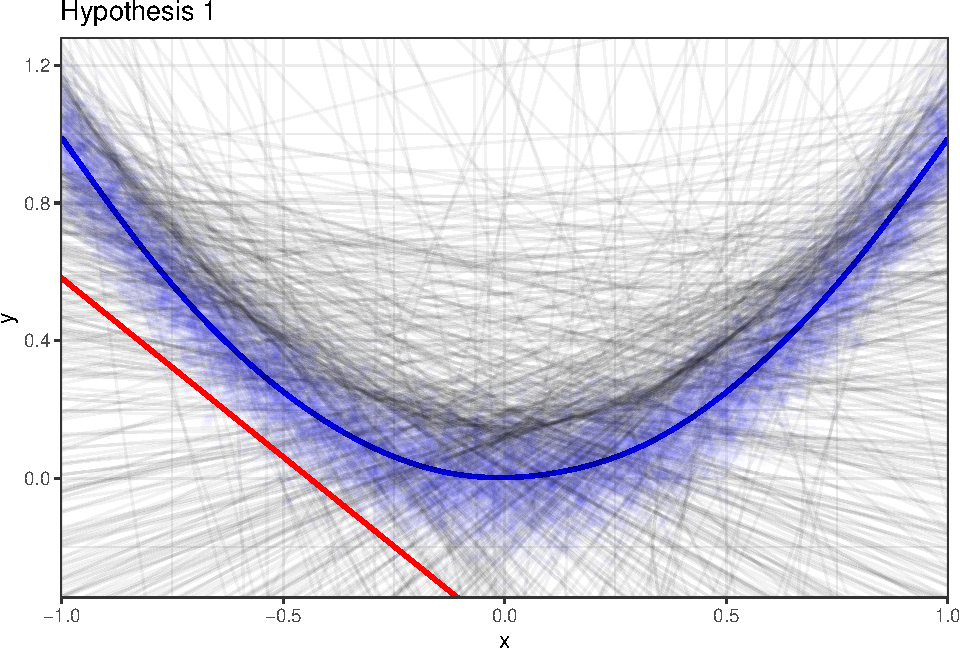
\includegraphics{hw4_files/figure-latex/unnamed-chunk-8-1.pdf}

\begin{Shaded}
\begin{Highlighting}[]
\CommentTok{# To verify the bias-variance trade-off rigorously, we examine the first model}
\NormalTok{OverallMSE_}\DecValTok{0}\NormalTok{ <-}\StringTok{ }\KeywordTok{mean}\NormalTok{(MSE_}\DecValTok{0}\NormalTok{)}
\NormalTok{bias <-}\StringTok{ }\KeywordTok{vector}\NormalTok{()}
\NormalTok{variance <-}\StringTok{ }\KeywordTok{vector}\NormalTok{()}
\ControlFlowTok{for}\NormalTok{ (i }\ControlFlowTok{in} \DecValTok{1}\OperatorTok{:}\DecValTok{20000}\NormalTok{)\{}
\NormalTok{  bias[i] <-}\StringTok{ }\NormalTok{(}\KeywordTok{mean}\NormalTok{(coef_}\DecValTok{0}\NormalTok{) }\OperatorTok{-}\StringTok{ }\NormalTok{x_out[i]}\OperatorTok{^}\DecValTok{2}\NormalTok{)}\OperatorTok{^}\DecValTok{2}
\NormalTok{\}}
\NormalTok{bias_}\DecValTok{0}\NormalTok{ <-}\StringTok{ }\KeywordTok{mean}\NormalTok{(bias)}
\ControlFlowTok{for}\NormalTok{ (i }\ControlFlowTok{in} \DecValTok{1}\OperatorTok{:}\DecValTok{500}\NormalTok{)\{}
\NormalTok{  variance[i] <-}\StringTok{ }\NormalTok{(}\KeywordTok{mean}\NormalTok{(coef_}\DecValTok{0}\NormalTok{) }\OperatorTok{-}\StringTok{ }\NormalTok{coef_}\DecValTok{0}\NormalTok{[i])}\OperatorTok{^}\DecValTok{2}
\NormalTok{\}}
\NormalTok{variance_}\DecValTok{0}\NormalTok{ <-}\StringTok{ }\KeywordTok{mean}\NormalTok{(variance)}
\CommentTok{# Display it tidily}
\NormalTok{model_}\DecValTok{0}\NormalTok{ <-}\StringTok{ }\KeywordTok{data.frame}\NormalTok{(}\StringTok{"OverallMSE"}\NormalTok{ =}\StringTok{ }\NormalTok{OverallMSE_}\DecValTok{0}\NormalTok{, }\StringTok{"Bias"}\NormalTok{ =}\StringTok{ }\NormalTok{bias_}\DecValTok{0}\NormalTok{, }\StringTok{"Var"}\NormalTok{ =}\StringTok{ }\NormalTok{variance_}\DecValTok{0}\NormalTok{)}
\NormalTok{model_}\DecValTok{0}
\end{Highlighting}
\end{Shaded}

\begin{verbatim}
##   OverallMSE       Bias        Var
## 1  0.1430415 0.08987592 0.04401978
\end{verbatim}

\begin{Shaded}
\begin{Highlighting}[]
\CommentTok{# If the decomposition is correct, it shall return 0}
\NormalTok{model_}\DecValTok{0}\OperatorTok{$}\NormalTok{OverallMSE }\OperatorTok{-}\StringTok{ }\NormalTok{model_}\DecValTok{0}\OperatorTok{$}\NormalTok{Bias }\OperatorTok{-}\StringTok{ }\NormalTok{model_}\DecValTok{0}\OperatorTok{$}\NormalTok{Var}
\end{Highlighting}
\end{Shaded}

\begin{verbatim}
## [1] 0.009145751
\end{verbatim}

\begin{Shaded}
\begin{Highlighting}[]
\NormalTok{OverallMSE_}\DecValTok{1}\NormalTok{ <-}\StringTok{ }\KeywordTok{mean}\NormalTok{(MSE_}\DecValTok{1}\NormalTok{)}
\NormalTok{bias <-}\StringTok{ }\KeywordTok{vector}\NormalTok{()}
\NormalTok{variance <-}\StringTok{ }\KeywordTok{rep}\NormalTok{(}\DecValTok{0}\NormalTok{, n_out)}
\ControlFlowTok{for}\NormalTok{ (i }\ControlFlowTok{in} \DecValTok{1}\OperatorTok{:}\DecValTok{20000}\NormalTok{)\{}
\NormalTok{  bias[i] <-}\StringTok{ }\NormalTok{(}\KeywordTok{mean}\NormalTok{(coef_1a) }\OperatorTok{+}\StringTok{ }\KeywordTok{mean}\NormalTok{(coef_1b)}\OperatorTok{*}\NormalTok{x_out[i] }\OperatorTok{-}\StringTok{ }\NormalTok{x_out[i]}\OperatorTok{^}\DecValTok{2}\NormalTok{)}\OperatorTok{^}\DecValTok{2}
\NormalTok{\}}
\NormalTok{bias_}\DecValTok{1}\NormalTok{ <-}\StringTok{ }\KeywordTok{mean}\NormalTok{(bias)}
\ControlFlowTok{for}\NormalTok{ (i }\ControlFlowTok{in} \DecValTok{1}\OperatorTok{:}\DecValTok{500}\NormalTok{)\{}
  \ControlFlowTok{for}\NormalTok{ (j }\ControlFlowTok{in} \DecValTok{1}\OperatorTok{:}\NormalTok{n_out)\{}
\NormalTok{    variance[i] =}\StringTok{ }\NormalTok{variance[i] }\OperatorTok{+}\StringTok{ }\NormalTok{((}\KeywordTok{mean}\NormalTok{(coef_1a) }\OperatorTok{+}\StringTok{ }\KeywordTok{mean}\NormalTok{(coef_1b)}\OperatorTok{*}\NormalTok{x_out[j] }\OperatorTok{-}\StringTok{ }\NormalTok{coef_1a[i] }\OperatorTok{-}\StringTok{ }\NormalTok{coef_1b[i]}\OperatorTok{*}\NormalTok{x_out[j])}\OperatorTok{^}\DecValTok{2}\NormalTok{)}\OperatorTok{/}\DecValTok{500}
\NormalTok{  \}}
\NormalTok{\}}

\NormalTok{variance_}\DecValTok{1}\NormalTok{ <-}\StringTok{ }\KeywordTok{mean}\NormalTok{(variance)}
\CommentTok{# Display it tidily}
\NormalTok{model_}\DecValTok{1}\NormalTok{ <-}\StringTok{ }\KeywordTok{data.frame}\NormalTok{(}\StringTok{"OverallMSE"}\NormalTok{ =}\StringTok{ }\NormalTok{OverallMSE_}\DecValTok{1}\NormalTok{, }\StringTok{"Bias"}\NormalTok{ =}\StringTok{ }\NormalTok{bias_}\DecValTok{1}\NormalTok{, }\StringTok{"Var"}\NormalTok{ =}\StringTok{ }\NormalTok{variance_}\DecValTok{1}\NormalTok{)}
\NormalTok{model_}\DecValTok{1}
\end{Highlighting}
\end{Shaded}

\begin{verbatim}
##   OverallMSE     Bias      Var
## 1    298.159 1.061858 297.0879
\end{verbatim}

\begin{Shaded}
\begin{Highlighting}[]
\CommentTok{# If the decomposition is correct, it shall return 0}
\NormalTok{model_}\DecValTok{1}\OperatorTok{$}\NormalTok{OverallMSE }\OperatorTok{-}\StringTok{ }\NormalTok{model_}\DecValTok{1}\OperatorTok{$}\NormalTok{Bias }\OperatorTok{-}\StringTok{ }\NormalTok{model_}\DecValTok{1}\OperatorTok{$}\NormalTok{Var }\OperatorTok{-}\StringTok{ }\FloatTok{0.01}
\end{Highlighting}
\end{Shaded}

\begin{verbatim}
## [1] -0.000808448
\end{verbatim}


\end{document}
